\documentclass[border=20pt]{standalone}
\usepackage[utf8]{inputenc}
\usepackage[T1]{fontenc}
\usepackage{tikz}
\usetikzlibrary{arrows.meta, shapes.geometric}

\begin{document}
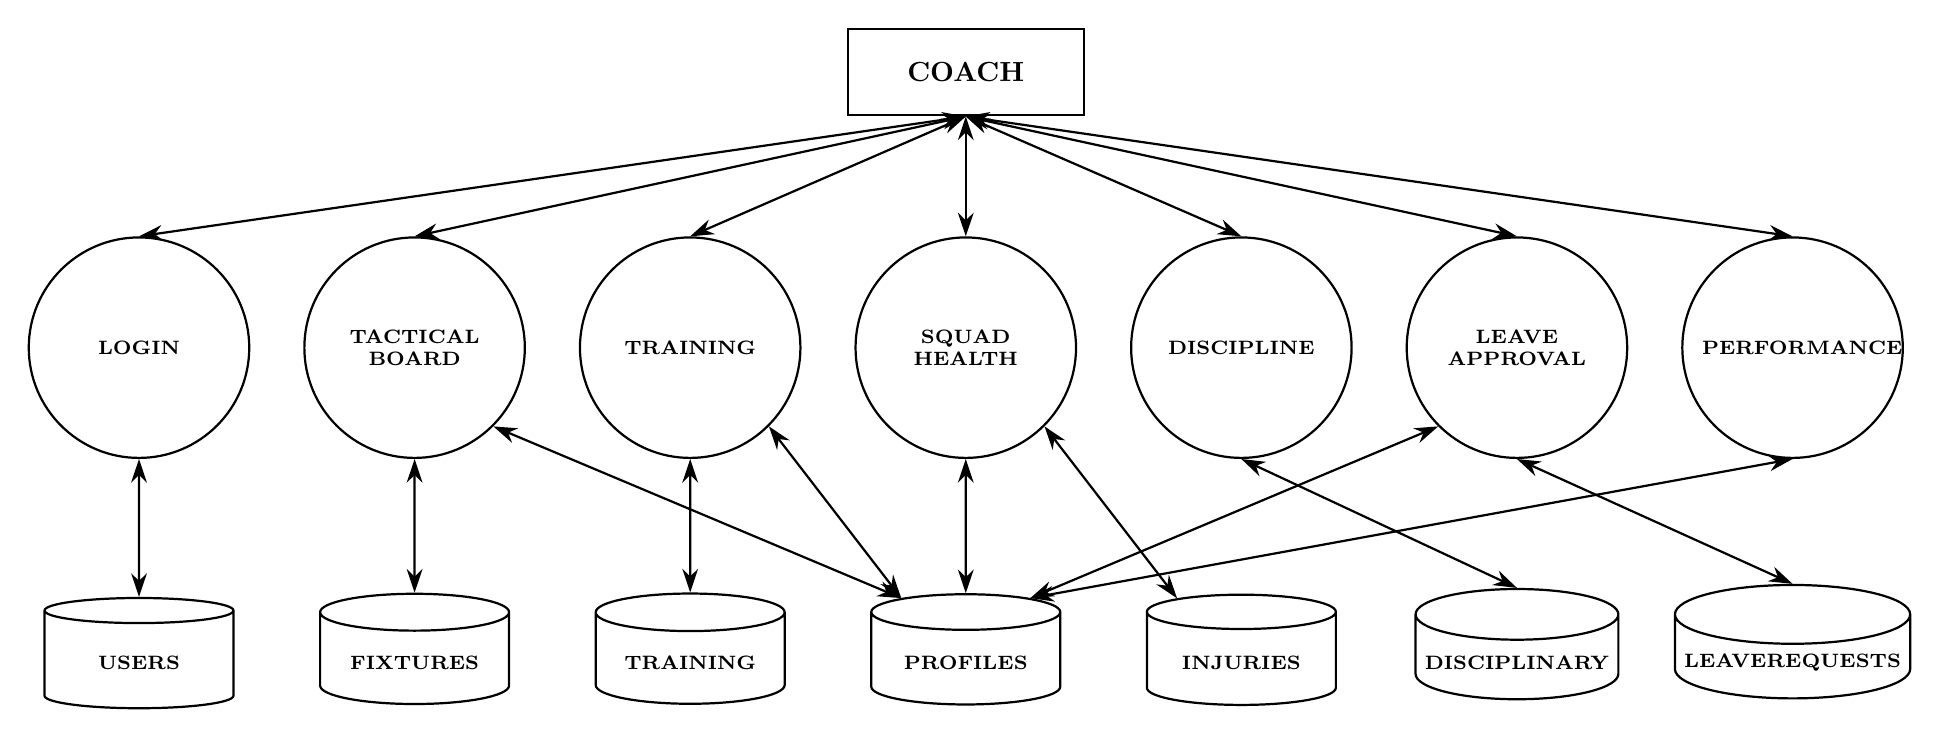
\begin{tikzpicture}[
  entity/.style={rectangle, draw, thick, minimum width=3cm, minimum height=1.1cm, font=\normalsize\bfseries, text centered},
  process/.style={circle, draw, thick, minimum size=2.8cm, font=\scriptsize\bfseries, text width=2.3cm, align=center},
  datastore/.style={cylinder, draw, thick, shape border rotate=90, aspect=0.25, minimum width=2.4cm, minimum height=1.4cm, font=\scriptsize\bfseries, text centered},
  biarr/.style={{Stealth[length=3mm, width=2mm]}-{Stealth[length=3mm, width=2mm]}, thick}
]

\node[entity] (coach) at (0, 6) {COACH};

\node[process] (p1) at (-10.5, 2.5)  {LOGIN};
\node[process] (p2) at (-7, 2.5)     {TACTICAL\\BOARD};
\node[process] (p3) at (-3.5, 2.5)   {TRAINING};
\node[process] (p4) at (0, 2.5)      {SQUAD\\HEALTH};
\node[process] (p5) at (3.5, 2.5)    {DISCIPLINE};
\node[process] (p6) at (7, 2.5)      {LEAVE\\APPROVAL};
\node[process] (p7) at (10.5, 2.5)   {PERFORMANCE};

\node[datastore] (d1) at (-10.5, -1.5) {USERS};
\node[datastore] (d2) at (-7, -1.5)    {FIXTURES};
\node[datastore] (d3) at (-3.5, -1.5)  {TRAINING};
\node[datastore] (d4) at (0, -1.5)     {PROFILES};
\node[datastore] (d5) at (3.5, -1.5)   {INJURIES};
\node[datastore] (d6) at (7, -1.5)     {DISCIPLINARY};
\node[datastore] (d7) at (10.5, -1.5)  {LEAVE\\REQUESTS};

\draw[biarr] (coach.south) -- (p1.north);
\draw[biarr] (coach.south) -- (p2.north);
\draw[biarr] (coach.south) -- (p3.north);
\draw[biarr] (coach.south) -- (p4.north);
\draw[biarr] (coach.south) -- (p5.north);
\draw[biarr] (coach.south) -- (p6.north);
\draw[biarr] (coach.south) -- (p7.north);

\draw[biarr] (p1.south) -- (d1.north);
\draw[biarr] (p2.south) -- (d2.north);
\draw[biarr] (p3.south) -- (d3.north);
\draw[biarr] (p4.south) -- (d4.north);
\draw[biarr] (p5.south) -- (d6.north);
\draw[biarr] (p6.south) -- (d7.north);
\draw[biarr] (p7.south) -- (d4.north east);

\draw[biarr] (p2.south east) -- (d4.north west);
\draw[biarr] (p4.south east) -- (d5.north west);
\draw[biarr] (p3.south east) -- (d4.north west);
\draw[biarr] (p6.south west) -- (d4.north east);

\end{tikzpicture}
\end{document}
